% Add `ngerman` to documentclass for German docs
\documentclass[12pt, a4paper]{article}
\usepackage{a4wide}
\usepackage{setspace}
\usepackage[utf8]{inputenc}

\usepackage{url}
\usepackage{hyperref}
\usepackage{minted}
\usemintedstyle{trac}

% inline code
\newcommand{\code}[1]{\texttt{#1}}

% Uncomment for German
%\usepackage[ngerman]{babel}

% For generating template dummy text
\usepackage{lipsum}

\usepackage{myColors}
\usepackage{myFooter}
\usepackage{myTitle}
\project{CS 432 Web Science}
\author{Derek Goddeau}
\title{Assignment One}
\supervisor{Michael L. Nelson}

\doublespace
\pagestyle{hacker}

\begin{document}
\maketitle

\newpage

\section{POST to a from with \code{curl}}

In order to submit \code{POST} data to a form using \code{curl} first
it must be ensured that the form accepts \code{POST} data. This can be
done by viewing the page source and verifying that the form tag has
\code{method="post"} as in the \href{https://nostarch.com}{nostarch.com}
search bar form tag shown somewhat abridged below.

\begin{minted}{html}

<form action="/" method="post" id="search-theme-form">
<input name="search_theme_form" value="" class="form-text"/>
<input name="op" value="Search" class="form-submit"/>
<input type="hidden" name="form_build_id" value="form-6Skwd"/>
<input type="hidden" name="form_id" value="search_theme_form"/>
</form>
\end{minted}

\noindent
In order to
craft the \code{curl} command the \code{-d} flag can be used along
with the \code{"name=value"} pattern for each input to the form
where \code{name} is copied from each input tag and \code{value}
is changed in the fields where the default values are not desired.

\begin{minipage}{\linewidth} % prevent splitting between pages
\vspace{2em}
\begin{minted}{bash}

curl -L -i -o results.html \
           -d "search_theme_form=$1" \
           -d "op=Search" \
           -d "form_build_id=form-6SkwdjCka872mUDOLyJspWzIHtkBGso7f5RMZ2fGr9U" \
           -d "form_id=search_theme_form" \
           https://www.nostarch.com/
\end{minted}
\vspace{2em}
\end{minipage}

\noindent
The command \code{curl\_post.sh car} will return
a page with the search results for "car" on \href{https://nostarch.com}
{nostarch.com}. Inspecting the output \code{results.html} the
\code{HTTP/1.1 200 OK} after a single redirect and lack of a 405
Method not allowed error means the request was successful.

\href{https://gitlab.com/datenstrom/cs532-s17/blob/master/assignments/assignment_one/curl/results.html}{
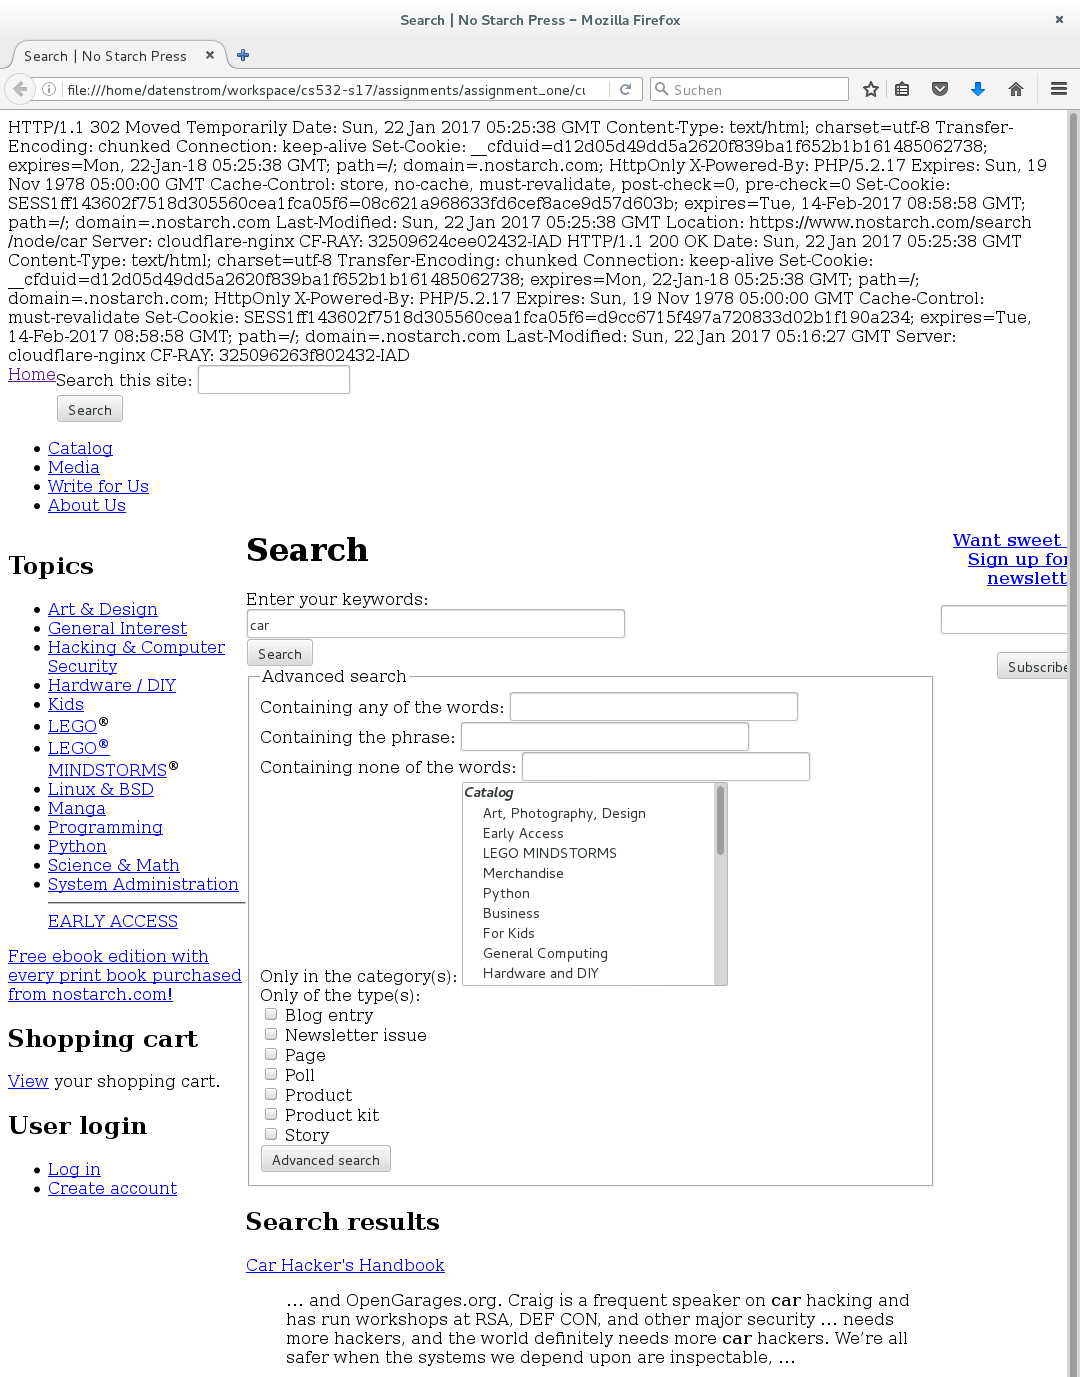
\includegraphics[width=\textwidth]{dia/curl_screenshot.png}
}

\section{A Python program that finds PDFs}

The \href{https://gitlab.com/datenstrom/cs532-s17/tree/master/assignments/assignment_one/common_house_spider}
{\code{Common House Spider}} can take any number of URIs as input
optionaly from a specified file with the \code{-f} flag. When searching
multiple URIs in parallel it may be useful to use the \code{-t} flag to
run it with multiple threads. It outputs all PDF files on the page and
their size.

%\begin{minipage}{\linewidth} % prevent splitting between pages
%    \vspace{2em}
%    \begin{minted}[mathescape,
%                   linenos,
%                   firstnumber=0,
%                   numbersep=5pt,
%                   gobble=1,
%                   frame=lines,
%                   framesep=2mm]{c}
%    /**
%     * Recursively calculate the factorial of n
%     *
%     * Only works for small numbers, meant to be a compact and
%     * clear function very close to the mathematical definition.
%     */
%    uintmax_t factorial(uintmax_t n) {
%        if(n == 1) return 1;
%        return(n * factorial(n - 1));
%    }
%    \end{minted}
%    \vspace{2em}
%\end{minipage}

\end{document}
